\chapter{Results and Discussion}

This chapter presents and analyzes the results obtained using the methodology
presented in the previous chapter.

\section{Performance}

%The results from using software only for hashing can be seen in table \ref{tab:Perf-SW}.
%The table shows the hashes per second for each active processor as number of processors are scaled up, beginning from Processor 0.
%The different rows are also grouped together, to highlight the distribution.
%The system reaches highest performance with only 3 active processors, and is saturated beyond this point.
%When using additional processors beyond this point, the hashing performance of each processor drops for each new that is added to the system.
%We believe that the stable number on the sum of hashes suggests that access to memory is the main bottleneck.

%It is interesting to note that performance drop for each processor on rows 0-2 no longer drops when fourth row has its processors added, one by one.
%It can also be observed that processor 10 has much greater performance.
%This is likely due to the SHMAC layout, combined with the current XY-routing.
%\todo{Should be improved by numbering the T-tiles in the figure, and cut down this sentence}Processor 10 is the T-tile on 2nd row, to the right edge, seen in figure \ref{fig:5x4}
%With XY-routing, there is no competition for routing between it and the DRAM-tile.
%There is either no competition for routing between the bottom row and the rest of the tiles either.
%This suggests that the mapping on SHMAC can improve or hamper performance, depending on the setup.
%Nevertheless, with memory as main bottleneck, a better mapping will have little effect on performance.
 
To establish a baseline for the performance gains obtained when using the accelerators,
a measurement of the performance when using software hashing was first obtained.

\subsection{Initial Software Results}

Using software-only hashing produced a best result of 16047 H/s. As can be seen
in the plot in figure \ref{fig:sw-scaling1}, however, adding more processors after the third produces no
noticeable additional performance gain. The reason for this is that all cores makes frequent
accesses to DRAM, when running the software algorithm, which causes the DRAM tile to quickly
become congested. The reason for these frequent accesses is probably due to the use of
many variables in the code as well as the effect of stack usage. Since the Turbo Amber core
uses a write-through cache, all memory writes ends up going to DRAM immediately which causes
additional congestion.

Another interesting effect to note in the results is how the XY routing affects the performance
of each tile. The more tiles that tries to access main memory through a tile, the less
performance that tile has; network congestion does, in other words, have a great impact on individual
tile performance.

This was especially obvious for processor tile 10, which is located on the end of row 3 with no
processors on either the left or right sides. This processor showed notably better performance than
any other processor in the grid. This is because its location means that no data to or from other processors
have to pass through the processor which gives it more time to process its own requests. In addition,
this processor can access all memory tiles without having to send or receive data through any other
processor tiles because of its location. The individual performance of each processor is noted in
appendix \ref{app:performance}, table \ref{tab:Full-Perf-SW1}.

\begin{figure}
	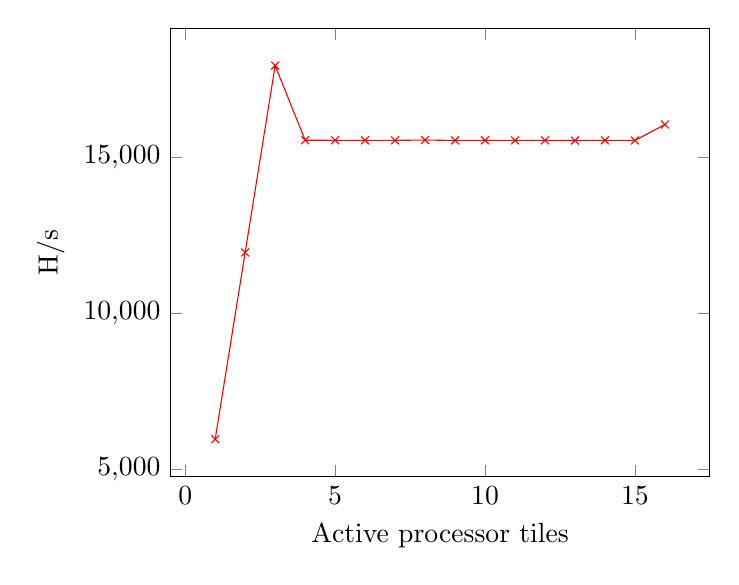
\begin{tikzpicture}
		\begin{axis}[
			xlabel=Active processor tiles,
			ylabel=H/s,
			scaled ticks=false]
		\addplot[color=red,mark=x] coordinates {
			(1, 5972)
			(2, 11950)
			(3, 17933)
			(4, 15543)
			(5, 15540)
			(6, 15539)
			(7, 15539)
			(8, 15549)
			(9, 15536)
			(10, 15541)
			(11, 15539)
			(12, 15537)
			(13, 15534)
			(14, 15540)
			(15, 15535)
			(16, 16047)
		};
		\end{axis}
	\end{tikzpicture}
	\caption{Scaling using software hashing}
	\label{fig:sw-scaling1}
\end{figure}

\subsection{Initial Hardware Results}
\label{sec:init-hw-results}

Need new results for hardware hashing! We totally forgot this last thursday.

Tables \ref{tab:Perf-SHA} and \ref{tab:Perf-SHADMA} shows the results when using the SHA-256 accelerator, without and with the DMA module enabled, respectively.
Only up to four processors where used, as adding in processors from the second row of processors when scaling up caused the application to crash.
It was discovered that this was likely because of an undocumented bug in the implementation of the scratchpad memory tile used.

Both tables shows that the sum of hashes has a near-linear increase when adding more tiles.
The individual perfomance of each processor varies, which is due to the same congestion effects observed when doing software hashing.
Using DMA shows the same trend, but with additionally increased performance for each tile.


\subsection{Alternative Software Results}
In order to obtain better results with regards to scaling, a new test design was created which works
around the scratchpad tile bug and places all CPU cores on the same line.

\begin{figure}
	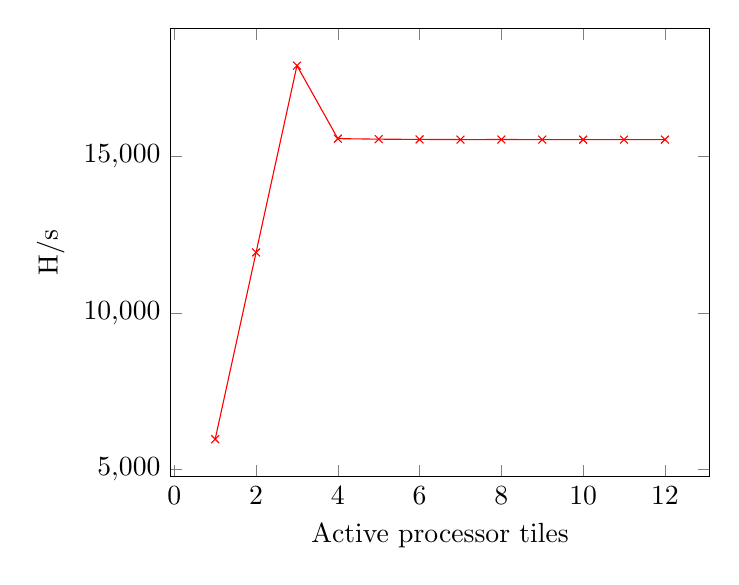
\begin{tikzpicture}
		\begin{axis}[
			xlabel=Active processor tiles,
			ylabel=H/s,
			scaled ticks=false]
		\addplot[color=red,mark=x] coordinates {
			(1, 5963)
			(2, 11930)
			(3, 17900)
			(4, 15566)
			(5, 15549)
			(6, 15541)
			(7, 15536)
			(8, 15537)
			(9, 15536)
			(10, 15534)
			(11, 15535)
			(12, 15536)
		};
		\end{axis}
	\end{tikzpicture}
	\caption{Scaling using software hashing, alternative architecture}
	\label{fig:sw-scaling2}
\end{figure}

\subsection{Alternative Hardware Results}
\section{Power and energy efficiency}

We must measure the power from the wall, before we can add anything here.

\section{Discussion about NoC efficiency}
\section{Discussion about SHMAC bugs}

\section{Discossion on various issues}
% Relevant stuffz copied from methodology:
%
%Caches were turned on for each testing, but a bug in the caches can cause several processors to halt over time, making measurements more difficult.
%Increased number of tiles in used increases the chance for a cache bug to happen.
%Additionally, no cache coherency protocol is implemented, and all shared data are therefore mapped to uncachable memory.
%Data hazard may be present when DMA and processor "shares" data, by loading or storing to the same address space in use.
%DMA may copy outdated data from memory that the cache has not yet written back, or overwrite data that the cache is not aware of.
%An operating system may handle data coherency where DMA involved, but since this project is done by running the software on bare metal, this security is absent.
%The Turbo Amber processor uses \todo{Must get it confirmed, and then source linked}write-through policy, so every data update is always written back to memory, \todo{Want to mention "reduced, but not removed", due to how our tests may go} reducing the possibility of data hazard, but not removing it.

%Interrupt handling for the hashing module is always in use, when the accelerator is used.

%The DMA Module is made only for transfering 32-bit words individually at a time.
%When transferring data internal on the tile (regular tile registers, hashing registers and DMA registers), this is all the local system requires, as the tile modules does not provide full blocks of \todo{Use of wishbone, with size 128, is not yet provided}4 words.
%\todo{Merely an assumption. We haven't tested this.}But when running the hashing in software only, the system is likely to achieve better data transfer rate using regular processor data transfer of 4 words, through the caches, since the current DMA would require 4 individual transfer, compared to the processor.

%The use of the included sub-module in the DMA that moves the bytes from high endian to little endian should further improve the performance and energy efficiency, by relieving the software for this task.
%The byte flip is done through combinatorical circuits, and should not add any extra execution time.
%Wihtout it, the software would require several independent operations, for loading in and shifting every single byte to the correct position of the word.

%Additionally, polling is used to control when a DMA is finished.
%Ideally, interrupt handling is preferable, but the interrupt handler for the DMA would not \todo{yet}work. 

